\chapter{Arkitektur}

I dette kapitel beskrives systemets arkitektur for hardware og software. Arkitekturens formål er at tildele roller til de enkelte hardware og software komponenter. Når denne arkitektur er fastsat er det muligt at designe systemet i detaljer. Arkitekturen illustreres i hardware-delen i Blok definition diagram (BDD), Internal blok diagram (IBD), en signaltabel og en blokbeskrivelse, der indeholder uddybende beskrivelse af blokkene i BDD'et. For Software-delens vedkommende anvendes også et BDD, som bruges til at illustrere hovedblokkene.

\section{Hardware}
\subsection{Blok definition diagram}

Dette afsnit omhandler arkitekturen af hardwaren, som anvendes til måling, analysering og visning af BI- og EMG-målinger. BDD'et på figur \ref{fig:arkitekturBDD} viser det overordnet system for SRM, som består af en HW-blok med tilhørende to HW-blokke. Disse to HW-blokke består af BI-sensor og EMG-sensor. EMG-sensoren består af to komponenter og BI-sensor består af seks blokke. Derudover er der en PC-blok og Analog Discovery blok. Disse blokke tilsammen udgør SRM.

\begin{figure}[H] 
\centering
{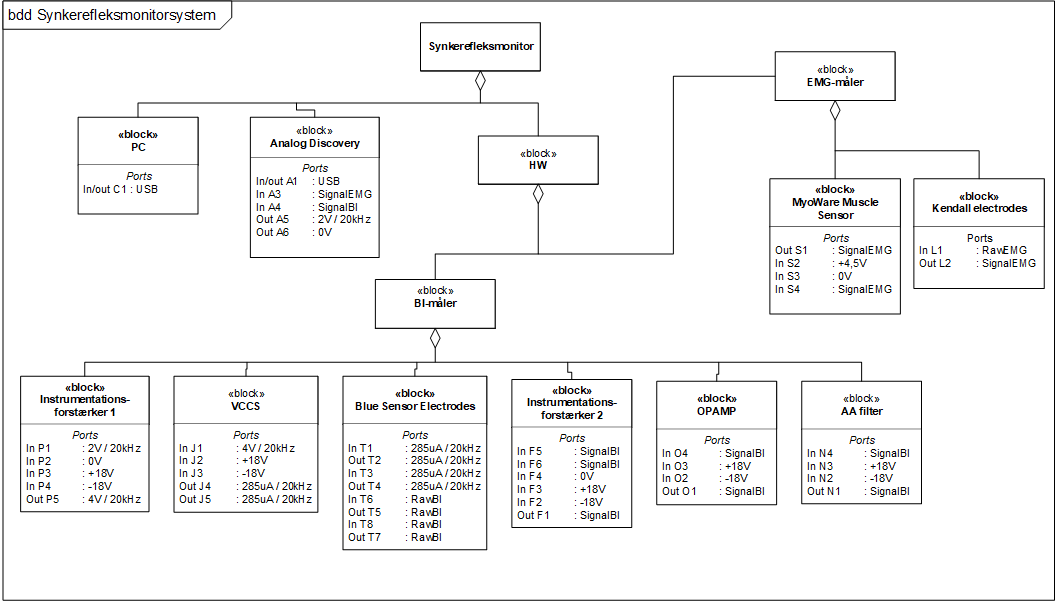
\includegraphics[width=13cm]
{Figure/BDD}}
\caption{Figuren viser de enkelte komponenter, som hardware-delen består af. Overordnet består
systemet af en BI-sensor, en EMG-sensor og Analog Discovery, der bruges til dataopsamling og som funktionsgenerator. Udover det er der en PC blok.}
\label{fig:arkitekturBDD}
\end{figure}



\subsection{Internal blok diagram}

IBD bruges til at vise den interne struktur og kommunikation mellem delsystemerne, se figur \ref{fig:ibdfigur}. SRM indeholder to uafhængige blokke, BI-sensoren og EMG-sensoren. De to blokke har kommunikation med blokken Analog Discovery og PC. 

Kommunikationsflowet for BI-sensor, starter ved at Analog Discovery generer et AC signal på 2 V til indgangen på Instrumentationsforstærker 1. Instrumentationsforstærker 1 forstærker signalet med faktor 2. Det forstærkede signal sendes videre til strømgeneratoren (VCCS), som genererer en konstant strøm. Denne strøm sendes til måleobjektet via to elektroder (Blue Sensor Electrodes). 

To yderligere elektroder (Blue Sensor Electrodes) påsættes på måleobjektet, for at måle en spændingsforskel. Biosignalet (spændingsforskellen) er svagt og støjfyldt (common mode støj), hvilket kræver at det bliver forstærket samt støjen reduceres. Signalet fra måleobjekt bliver forstærket af instrumentationsforstærkeren samtidig med, at der fjernes common mode støj. Herefter bliver signalet yderligere forstærket af en opamp. Efter denne forstærkning bliver signalet filtreret i et anti-aliaseringsfilter, der dæmper frekvenskomponenter over Nyquist-frekvensen. 

Til sidst sendes signalet til dataopsamlingsenheden Analog Discovery, der kommunikerer med en PC, hvor signalet bliver analyseret og vist. BI-sensoren bliver forsynet med en eksitationsspænding på $\pm$18 V.

EMG-sensoren består af en Myoware Muscle Sensor og tre elektroder, der måler muskelaktiviteten over det valgte segment på måleobjektet. Det målte signal opsamles også vha. Analog Discovery. Myoware Muscle Sensor forsynes med en eksitationsspænding på $+$4,5 V.


\begin{figure}[H]
\centering
{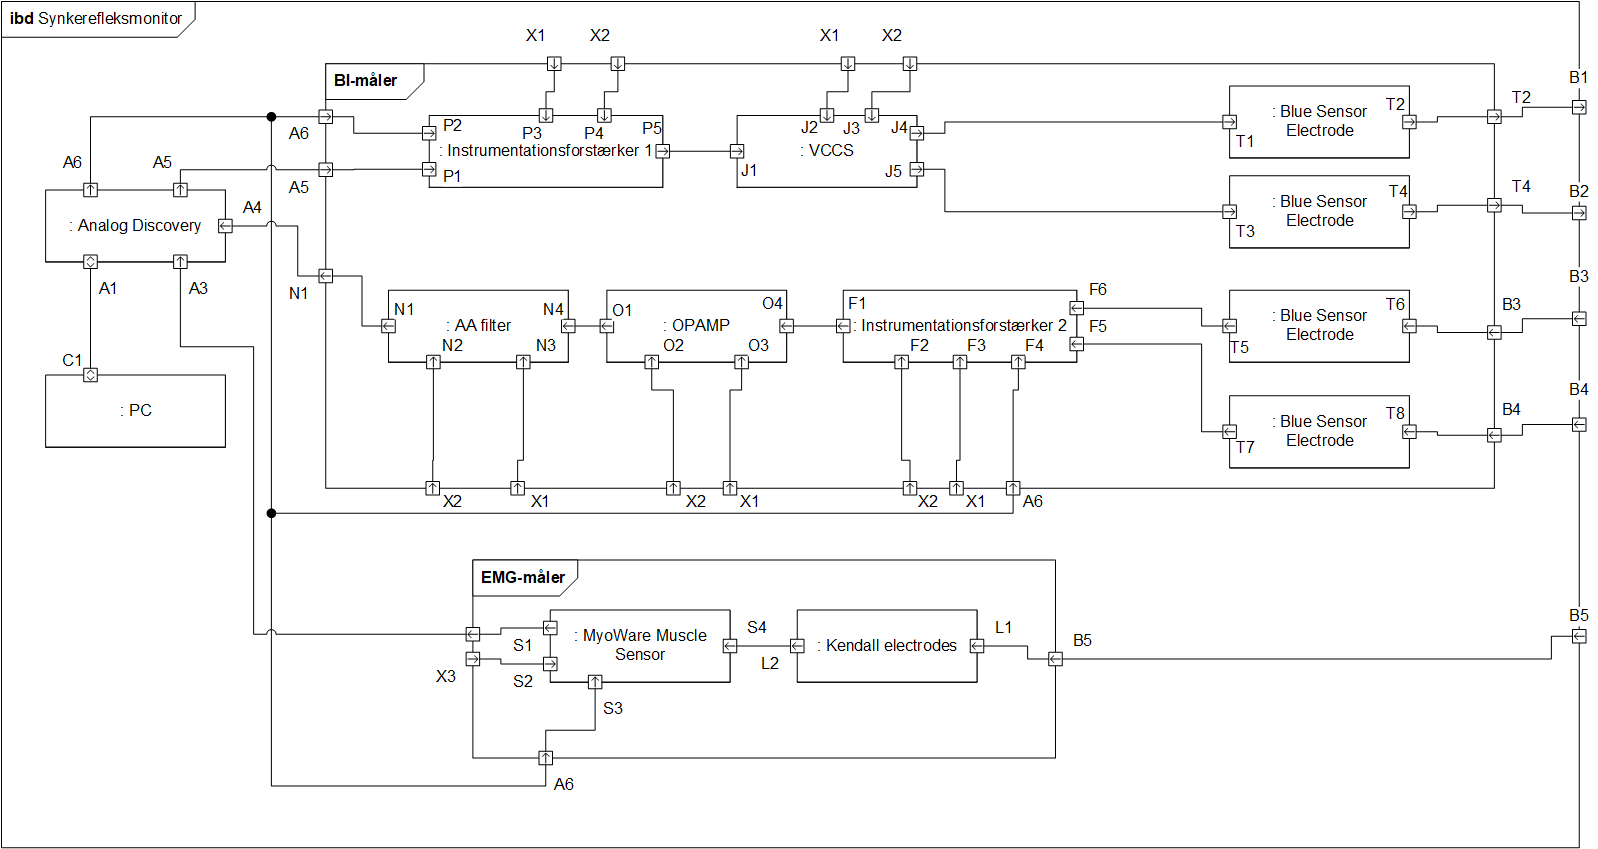
\includegraphics[width=\linewidth]
{Figure/IBD}}
\caption{Figuren viser et internt blokdiagram, der illustrer den interne relation og signalflow mellem delsystemer for SRM. Hver port repræsenterer en fysisk grænseflade på blokken. Overordnet set indeholder diagrammet to hovedblokke med hver deres subkomponenter. Den ene af de store blokke repræsenter en BI-sensor og den anden blok repræsenter en EMG-sensor.}
\label{fig:ibdfigur}
\end{figure}


\subsection{Blokbeskrivelse}

Da BDD og IBD ikke alene kan forklare blokkenes og signalernes funktionalitet, kan disse forklares præcist vha. af forklarende tekst i tabeller. Tabel \ref{tab:BlokBeskr} viser blokbeskrivelsen for to blokke, samt deres signaltyper og navne. Funktionerne for alle blokkene kan læses i  \nameref{bilag4}.


\begin{table}[H]
\centering
\begin{tabularx}{\textwidth}{l|X|X|X}
\hline
\textbf{Blok-navn}                        & \textbf{Funktions-beskrivelse}  & \textbf{Signaler} & \textbf{Kommentar} \\  \hline

PC & Behandler input fra Analog Discovery.  &  USB & Dataoverførelse med Analog Discovery   \\ \cline{3-4} \hline


Analog Discovery & Fungerer som funktionsgenerator, og  A/D-konverter. Den kommunikerer også med PC'en.  &  USB & Dataoverførelse med Analog Discovery   \\ \cline{3-4}

 	 
 	 &  & SignalEMG & Indgangssignal  \\ \cline{3-4}
 	 
 	 &  & SignalBI & Indgangssignal  \\ \cline{3-4}
 	 &  & $   ${2V,20kHz} & Funktionsgenerator  \\ \cline{3-4}
 	 &  & $   ${0V} & Reference  \\ \cline{3-4} \hline
 	 
\end{tabularx}
\caption{Tabellen viser blokbeskrivelse for to blokke.} 
\label{tab:BlokBeskr}
\end{table}

\pagebreak

Til slut fuldendes grænsefladebeskrivelsen i en detaljeret signaltabel, tabel \ref{tab:signaltabel}. Signaltabellens anvendelse er tiltænkt når grænsefladerne skal designes. Da dette kun er et udpluk henvises der til den komplette signaltabel i \nameref{bilag4}.



\begin{table}[H]
\centering
\begin{tabularx}{\textwidth}{l|X|X|X|X|X}
\hline

\textbf{Signal-navn}  & \textbf{Funktion}  & \textbf{Område} & \textbf{Port 1}      & \textbf{Port 2}  & \textbf{Kommentar} \\ \cline{4-6} \hline


0V & Reference til analoge spændinger  &   & Analog Discovery, A6  & Instrumenta-tions-forstærker 1, P2  &  stel   \\ \cline{4-6}

 &  &   &  Analog Discovery, A6 & Instrumenta-tions-forstærker 2, F4 & \\ \cline{4-6} 
 
 &  &   &  Analog Discovery, A6 & MyoWare Muscle Sensor, S3 & \\ \cline{4-6}

 \hline
4,5V & Forsynings- spænding til MyoWare Muscle Sensor  &  4,0-4,5 V & Analog Discovery, A2 & MyoWare Muscle Sensor, S2&     \\ \cline{4-6}	\hline

\end{tabularx}
\caption{Figuren viser signalbeskrivelsen for to signaler.}
\label{tab:signaltabel}
\end{table}



\section{Software}
\subsection{Blok definition diagram}

Dette afsnit omhandler arkitekturen af softwaren, som anvendes til måling, analysering og visning af BI- og EMG-målinger. Softwarens arkitektur er drevet af de use cases, som er beskrevet i \nameref{bilag1}. Derfor udformes et BDD på baggrund af disse use cases, som består af en parent-blok og fire child-blokke, se figur \ref{fig:SWIBD}. 

I dette bachelorprojekt anvendes udviklingsværktøjet Matlab til at realisere projektes software-del. Udover Matlab kode udvikles en GUI i selv samme udviklingsværktøj. Denne GUI indeholder objekter f.eks. knapper, tekstfelter og tekstbokse m.m. Når Matlab GUI anvendes, skrives programmets funktionaliteter i funktioner, som så kaldes fra objekternes autogeneret callback funktioner, når de skal anvendes. Child-blokkene repræsenterer callback funktionerne og de er oprettet i hovedfilen synkerefleksmonitor.m. Funktionerne i child-blokkene består af selvstændige m-filer. Hver funktion behandler bestemte opgaver, samt interagere med de andre funktioner.

Softwaren fungerer, ved at sundhedspersonalet initialiserer kodeeksekveringen, ved at starte programmet Synkerefleksmonitor. Ved at aktivere knappen \textit{"Start Measurements"}, foretages der to målinger simultant. Disse målinger analyseres og vises i en graf til sundhedspersonalet. Nu er det muligt at få målingerne gemt via knappen \textit{"Save Measurements"}. Målingerne bliver gemt lokalt på computeren. De gemte målingerne kan hentes frem via knappen \textit{"Load Measurements"}. Rækkefølgen hvori programmets kode eksekveres beskrives vha. et sekvens diagram, som kan læses i \nameref{bilag5}.



\begin{figure}[H]
\centering
{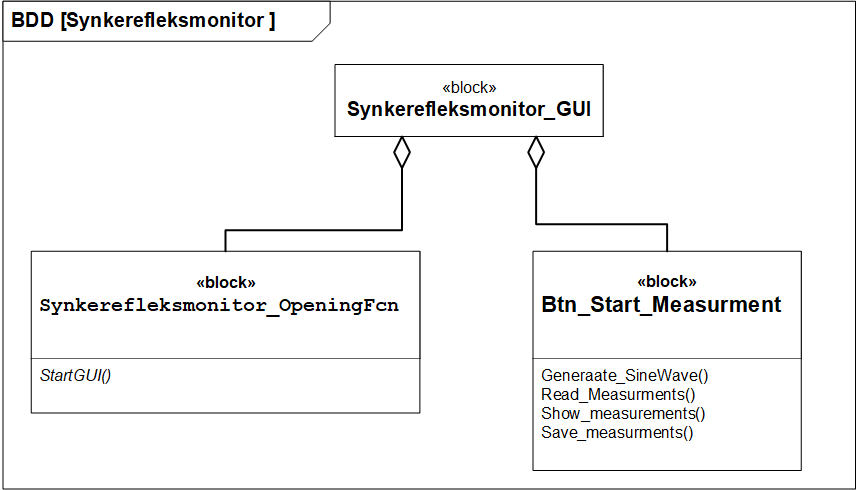
\includegraphics[width=\linewidth]
{Figure/SWIBD}}
\caption{Figuren viser block definition diagrammet for det ønsket software. Diagrammet indeholder en hovedblok, der består af fire andre blokke, som hver indeholder Matlab funktioner. Disse funktioner tilsammen måler, analyserer og viser to målinger simultant.}
\label{fig:SWIBD}
\end{figure}

